\documentclass[journal,5pt,twocolumn]{IEEEtran}
%
\makeatletter
\makeatother
\usepackage{setspace}
\usepackage{gensymb}
\usepackage{xcolor}
\usepackage{caption}
%\usepackage{stackengine}
%\usepackage{subcaption}
%\doublespacing
\singlespacing



\usepackage{graphicx}
\graphicspath{ {./images}  }
%\usepackage{amssymb}
%\usepackage{relsize}
\usepackage[cmex10]{amsmath}
\usepackage{mathtools}
%\usepackage{amsthm}
\interdisplaylinepenalty=2500
%\savesymbol{iint}
%\usepackage{txfonts}
%\restoresymbol{TXF}{iint}
\usepackage{wasysym}
\usepackage{amsthm}
\usepackage{mathrsfs}
\usepackage{txfonts}
\usepackage{stfloats}
\usepackage{cite}
\usepackage{cases}
\usepackage{mathtools}
\usepackage{subfig}
\usepackage{enumerate}	
\usepackage{enumitem}
\usepackage{amsmath}
%\usepackage{xtab}
\usepackage{longtable}
\usepackage{multirow}
%\usepackage{algorithm}
%\usepackage{algpseudocode}
\usepackage{enumitem}
\usepackage{mathtools}
\usepackage[colorlinks=true, allcolors=blue]{hyperref}
%\usepackage{iithtlc}
\usepackage{tikz}
\usetikzlibrary{shapes,arrows}

%\usetikzlibrary{arrows.meta,calc,positioning}
%\usepackage[framemethod=tikz]{mdframed}
\usepackage{listings}
    \usepackage[latin1]{inputenc}                                 %%
    \usepackage{color}                                            %%
    \usepackage{array}                                            %%
    \usepackage{longtable}                                        %%
    \usepackage{calc}                                             %%
    \usepackage{multirow}                                         %%
    \usepackage{hhline}                                           %%
    \usepackage{ifthen}                                           %%
  %optionally (for landscape tables embedded in another document): %%
    \usepackage{lscape}     


%\usepackage{stmaryrd}


%\usepackage{wasysym}
%\newcounter{MYtempeqncnt}
\DeclareMathOperator*{\Res}{Res}
%\renewcommand{\baselinestretch}{4}
%\setcounter{secnumdepth}{4}
\renewcommand\thesection{\arabic{section}}
\renewcommand\thesubsection{\thesection.\arabic{subsection}}
\renewcommand\thesubsubsection{\thesubsection.\arabic{subsubsection}}
%\renewcommand\thesubsubsubsection{\thesubsubsection.\arabic{subsubsubsection}}

%\renewcommand\thesectiondis{\arabic{section}}
%\renewcommand\thesubsectiondis{\thesectiondis.\arabic{subsection}}
%\renewcommand\thesubsubsectiondis{\thesubsectiondis.\arabic{subsubsection}}
%\renewcommand\thesubsubsubsectiondis{\thesubsubsectiondis.\arabic{subsubsubsection}}
% correct bad hyphenation here
\hyphenation{Future Wireless communications}

%\lstset{
%language=C,
%frame=single, 
%breaklines=true
%}

%\lstset{
	%%basicstyle=\small\ttfamily\bfseries,
	%%numberstyle=\small\ttfamily,
	%language=Octave,
	%backgroundcolor=\color{white},
	%%frame=single,
	%%keywordstyle=\bfseries,
	%%breaklines=true,
	%%showstringspaces=false,
	%%xleftmargin=-10mm,
	%%aboveskip=-1mm,
	%%belowskip=0mm
%}

%\surroundwithmdframed[width=\columnwidth]{lstlisting}
\def\inputGnumericTable{}                                 %%

\lstset{
%language=python,
frame=single, 
breaklines=true,
columns=fullflexible
}

 

\begin{document}
%
\tikzstyle{block} = [rectangle, draw,
text width=7em, text centered, minimum height=4em]
\tikzstyle{sum} = [draw, circle, node distance=3cm]
\tikzstyle{input} = [coordinate]
\tikzstyle{output} = [coordinate]
\tikzstyle{pinstyle} = [pin edge={to-,thin,black}]
\tikzstyle{line} = [draw, -latex']
\theoremstyle{definition}
\newtheorem{theorem}{Theorem}[section]
\newtheorem{problem}{Problem}
\newtheorem{proposition}{Proposition}[section]
\newtheorem{lemma}{Lemma}[section]
\newtheorem{corollary}[theorem]{Corollary}
\newtheorem{example}{Example}[section]
\newtheorem{definition}{Definition}[section]
%\newtheorem{algorithm}{Algorithm}[section]
%\newtheorem{cor}{Corollary}
\newcommand{\BEQA}{\begin{eqnarray}}
\newcommand{\EEQA}{\end{eqnarray}}
\newcommand{\define}{\stackrel{\triangle}{=}}
\bibliographystyle{IEEEtran}
%\bibliographystyle{ieeetr}
\providecommand{\nCr}[2]{\,^{#1}C_{#2}} % nCr
\providecommand{\nPr}[2]{\,^{#1}P_{#2}} % nPr
\providecommand{\mbf}{\mathbf}
\providecommand{\pr}[1]{\ensuremath{\Pr\left(#1\right)}}
\providecommand{\qfunc}[1]{\ensuremath{Q\left(#1\right)}}
\providecommand{\sbrak}[1]{\ensuremath{{}\left[#1\right]}}
\providecommand{\lsbrak}[1]{\ensuremath{{}\left[#1\right.}}
\providecommand{\rsbrak}[1]{\ensuremath{{}\left.#1\right]}}
\providecommand{\brak}[1]{\ensuremath{\left(#1\right)}}
\providecommand{\lbrak}[1]{\ensuremath{\left(#1\right.}}
\providecommand{\rbrak}[1]{\ensuremath{\left.#1\right)}}
\providecommand{\cbrak}[1]{\ensuremath{\left\{#1\right\}}}
\providecommand{\lcbrak}[1]{\ensuremath{\left\{#1\right.}}
\providecommand{\rcbrak}[1]{\ensuremath{\left.#1\right\}}}
\theoremstyle{remark}
\newtheorem{rem}{Remark}
\newcommand{\sgn}{\mathop{\mathrm{sgn}}}
\providecommand{\abs}[1]{\left\vert#1\right\vert}
\providecommand{\res}[1]{\Res\displaylimits_{#1}} 
\providecommand{\norm}[1]{\lVert#1\rVert}
\providecommand{\mtx}[1]{\mathbf{#1}}
\providecommand{\mean}[1]{E\left[ #1 \right]}
\providecommand{\fourier}{\overset{\mathcal{F}}{ \rightleftharpoons}}
%\providecommand{\hilbert}{\overset{\mathcal{H}}{ \rightleftharpoons}}
\providecommand{\system}{\overset{\mathcal{H}}{ \longleftrightarrow}}
	%\newcommand{\solution}[2]{\textbf{Solution:}{#1}}
\newcommand{\solution}{\noindent \textbf{Solution: }}
\newcommand{\myvec}[1]{\ensuremath{\begin{pmatrix}#1\end{pmatrix}}}
\providecommand{\dec}[2]{\ensuremath{\overset{#1}{\underset{#2}{\gtrless}}}}
\DeclarePairedDelimiter{\ceil}{\lceil}{\rceil}
%\numberwithin{equation}{subsection}
\numberwithin{equation}{section}
%\numberwithin{problem}{subsection}
%\numberwithin{definition}{subsection}
%\makeatletter
%\@addtoreset{figure}{section}
%\makeatother
\let\StandardTheFigure\thefigure
%\renewcommand{\thefigure}{\theproblem.\arabic{figure}}
%\renewcommand{\thefigure}{\thesection}
%\numberwithin{figure}{subsection}
%\numberwithin{equation}{subsection}
%\numberwithin{equation}{section}
%\numberwithin{equation}{problem}
%\numberwithin{problem}{subsection}
%\numberwithin{problem}{section}
%%\numberwithin{definition}{subsection}
%\makeatletter
%\@addtoreset{figure}{problem}
%\makeatother
%\makeatletter
%\@addtoreset{table}{problem}
%\makeatother
\let\StandardTheFigure\thefigure
\let\StandardTheTable\thetable
\let\vec\mathbf
%%\renewcommand{\thefigure}{\theproblem.\arabic{figure}}
%\renewcommand{\thefigure}{\theproblem}
%%\numberwithin{figure}{section}
%%\numberwithin{figure}{subsection}
\def\putbox#1#2#3{\makebox[0in][l]{\makebox[#1][l]{}\raisebox{\baselineskip}[0in][0in]{\raisebox{#2}[0in][0in]{#3}}}}
     \def\rightbox#1{\makebox[0in][r]{#1}}
     \def\centbox#1{\makebox[0in]{#1}}
     \def\topbox#1{\raisebox{-\baselineskip}[0in][0in]{#1}}
     \def\midbox#1{\raisebox{-0.5\baselineskip}[0in][0in]{#1}}
\title{ 
%	\logo{
Golioth with PSoC 6 Wi-Fi BT  Kit 
%	}
}
\author{Yadati Krishna \& Darla Pratheek}% <-this % stops a space
% make the title area
\maketitle
\tableofcontents
\section{\textbf{Introduction}}
Golioth is an IoT platform that provides cloud services for embedded devices. Colloquially, to solve the impedance mismatch between hardware and cloud engineering teams. Golioth is purpose-built for you and the hardware you develop. Enable everything that your devices need from the cloud, including device messaging, security, updates, analytics, and more.
\section{\textbf{Golioth-Platform Overview}}
To prepare your Golioth account to communicate directly with your hardware devices.The following steps are involved:
%\begin{enumerate}
%\item Register for your account on {\href{https://golioth.io/}{Golioth}}.
%\item Add a project and provision your first device.
%\end{enumerate}

\subsection{\textbf{Registration \& Wizard}}
To begin using Golioth please register for an account at {\href{https://golioth.io/}{Golioth}}.
Once registered, you can review the terms of service and continue to the Wizard that guides you through provisioning your first device.\\
Follow These steps:
\vspace{3mm}

\begin{enumerate}
\item {\textbf{Project name:}}
Enter a Project Name of your choosing\\

\vspace{10mm}

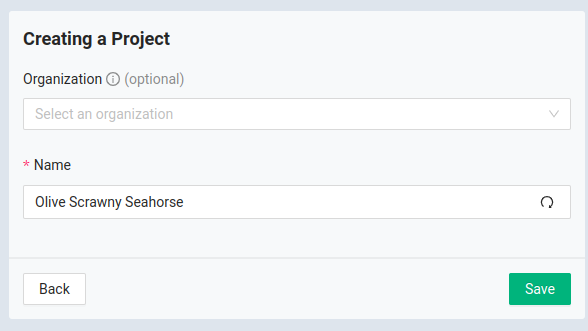
\includegraphics[width=0.5\textwidth]{../Pictures/create-proj.png} 
\vspace{5mm}
\item {\textbf{Device name:}}
Enter a Device Name\\


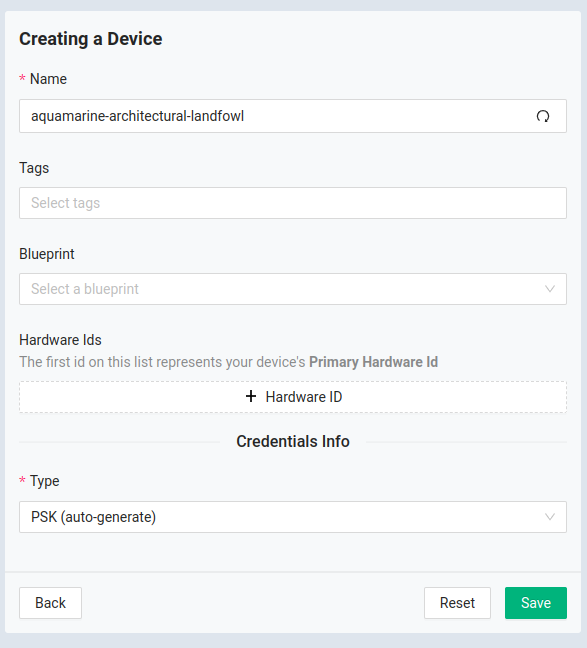
\includegraphics[width=0.5\textwidth]{../Pictures/create-device.png} 
\vspace{10mm}
\item {\textbf{Device credentials:}}
The Identity of this device is automatically populated from the device name with -id and @project-name appended,A Pre-Shared Key (PSK) is automatically generated. This is a password that will authenticate this device to the Golioth Cloud.



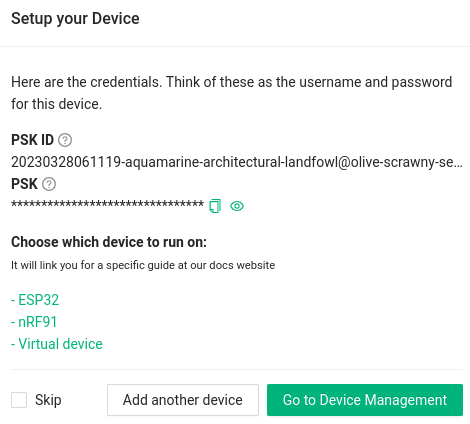
\includegraphics[width=0.4\textwidth]{../Pictures/setup.png} 
\end{enumerate}

\subsection{\textbf{Manage Devices}}
Use the Golioth Console to create a new device.\\

\vspace{5mm}

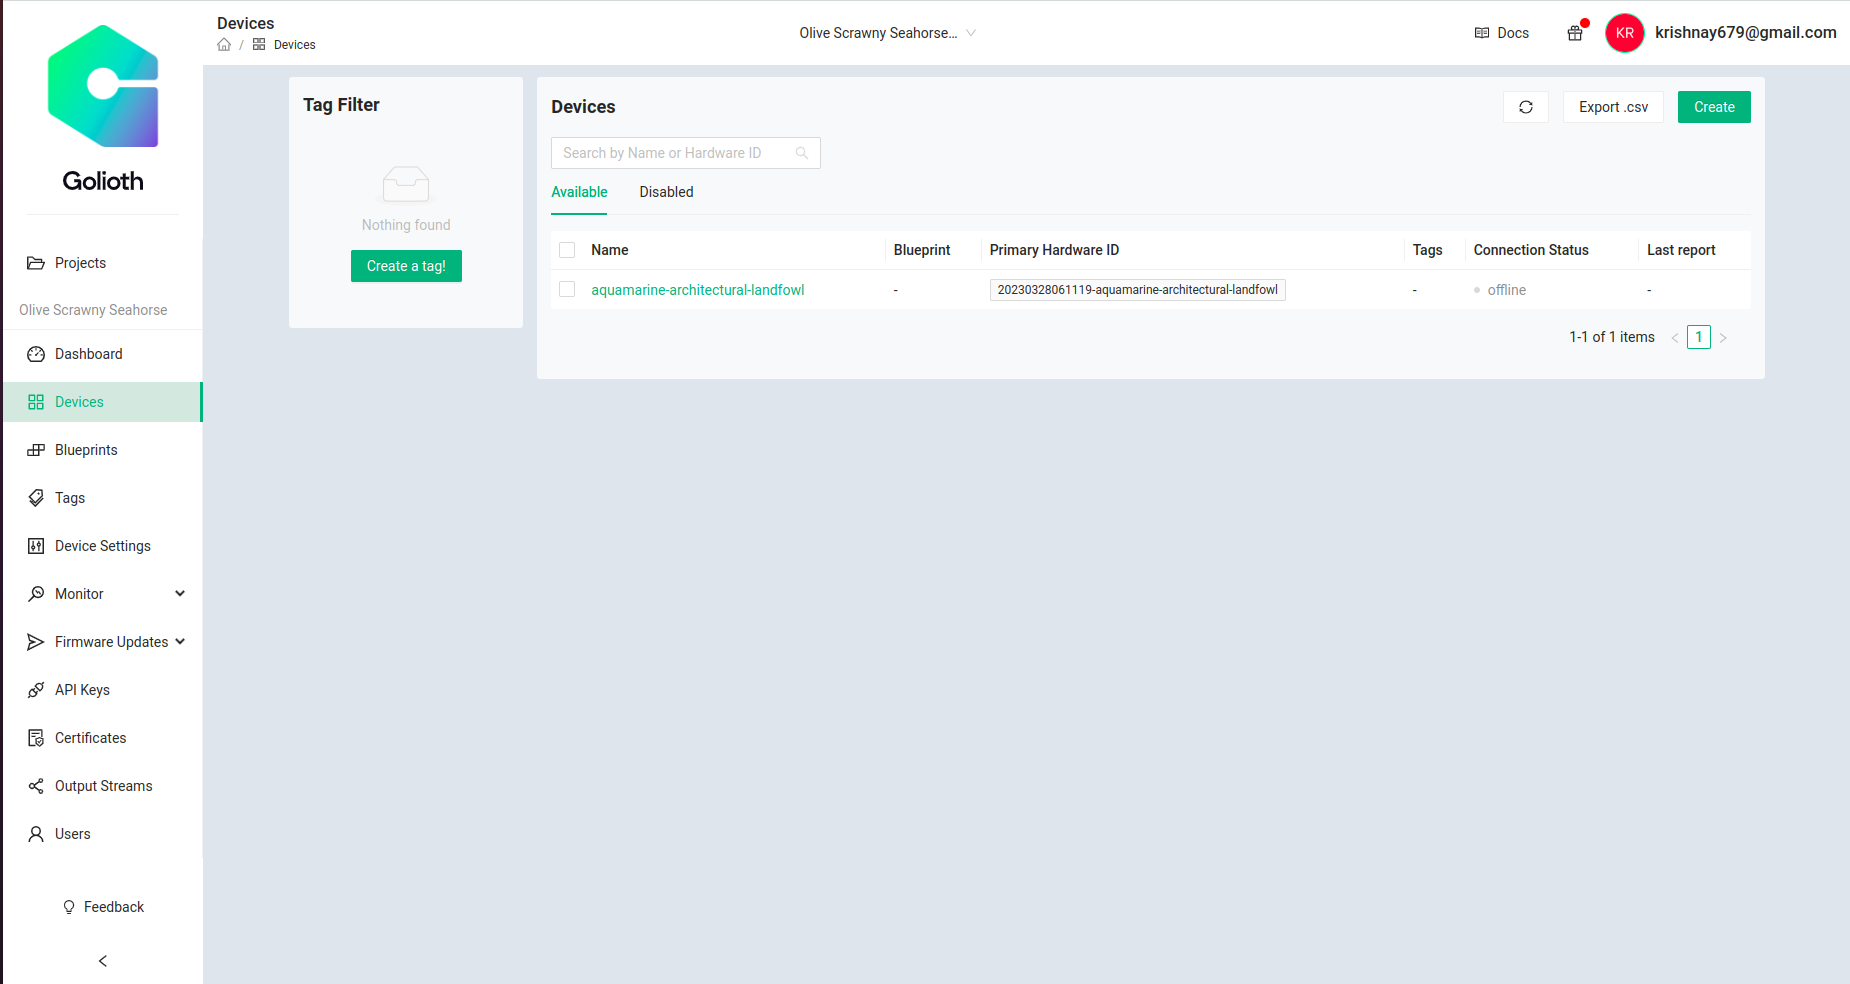
\includegraphics[width=0.45\textwidth]{../Pictures/manage-device.png} \\

In the center at the top of the console widow the currently selected project is shown. On the left sidebar we can use the Devices option to list this project's devices. Here we see the device that was created by the quickstart wizard.

\section{\textbf{Board Support Tiers}}
Golioth has three levels of board support: Continuously Verified, Verified, and Unverified.
\subsection{\textbf{Continuously Verified Boards}}
\raggedright A continuously verified board is highly recommended for new users that want to try out Golioth,is tested on every release of the Golioth Zephyr SDK,is regularly tested and used by the Golioth development team \& has first class support and maintenance from Golioth.
The set of boards in this category covers commonly used connectivity options including WiFi, cellular, and Thread. Additionally, these boards cover common MCUs, such as the ESP32 and nRF91.
\subsection{\textbf{Verified Boards}}
\raggedright A verified board is tested and confirmed to work with Golioth,is tested less frequently than continuously verified boards. 
This means it was tested on an older version of the Golioth Zephyr SDK, but may not have been tested on the most recent commits \& is supported and maintained by the Golioth development team.Boards in this category cover a wider range of MCUs and peripherals.
\subsection{\textbf{Unverified Boards}}
\raggedright An unverified board has not yet been verified to work with Golioth.It's very possible that the board may work well with Golioth, but it has not yet been tested by the Golioth team.Check if the board is in {\href{https://docs.zephyrproject.org/latest/boards/index.html}{List of supported boards}}. If it's in the list, there's a good chance it will work with Golioth with low development effort.
\section{\textbf{Golioth with Esp32}}
\raggedright The ESP32 is a Wi-Fi and Bluetooth combination chip from Espressif Systems. There are multiple versions of the chip, with the most recent versions running in different configurations of core types, up to and including a RISC V core (on the ESP32-C3).The Espressif team has built-in support for Zephyr. This, in combination with the low cost and wide availability of the chips, has led to the ESP32 being one of the first platforms that Golioth has chosen to support.
\subsection{\textbf{Setup Esp-IDF for Esp32}}
The Required installations for Esp-IDF is given in {\href{https://github.com/KrishnaYadati/Golioth-PSoC/blob/main/docs/esp-idf_installation.txt}{Github}}.
\begin{enumerate}
\item Install all the required commands as given from the above link.
\item Build and Flash the code as given in the link above.
\item Then open monitor using monitor command "idf.py monitor".
\item Open your golioth account and notice logs you can see this\\
\vspace{5mm}

  \includegraphics[width=0.5\textwidth]{../Pictures/Screenshot from 2023-03-27 22-18-29.png} 
  
\end{enumerate}
\subsection{\textbf{Setup Zephyr for Esp32}}
Golioth can be added to a device with Device SDKs which are based on different embedded Operating Systems. Currently Golioth targets the Zephyr Project and builds upon the APIs \& tools of Zephyr.\\
The Required installations are given in {\href{https://github.com/KrishnaYadati/Golioth-PSoC/blob/main/docs/zephyr-esp32_installation.txt}{Github}}.
\begin{enumerate}
\item Install all the required commands as given from the above link.
\item Build and Flash the code as given in the link above.
\item Then open monitor using screen command "screen /dev/ttyUSB0 115200".
\item Open your golioth account and notice logs you can see as in Esp32\\
%\vspace{5mm}

 % \includegraphics[width=0.5\textwidth]{../Pictures/Screenshot from 2023-03-27 22-18-29.png} 
  
\end{enumerate}

\section{\textbf{Golioth with PSoC}}
 \raggedright Infineon's PSoC 6 chips are feature rich 32-bit Arm microcontrollers. Paired with the Infineon's 4343W, it a perfect platform for IoT device builders, and exactly the kind of constrained device that Golioth was built for.Golioth now supports Infineon parts via the ModusToolbox.
\subsection{\textbf{ModusToolBox}}
ModusToolbox (MTB) is a software support tool from Infineon Technologies. It includes partner SDKs alongside the company's officially supported IDEs, drivers, and examples. You can pull in the Golioth example and all dependencies using the Eclipse IDE that is included in MTB, or via the command line tool.
\subsection{\textbf{Install ModusToolBox}}
\begin{enumerate}
\item Install {\href{https://www.infineon.com/cms/en/design-support/tools/sdk/modustoolbox-software/?redirId=VL1299}{ModusToolBox}} Software as per your operating system.
\item Extract the files and do all the necessary installations(Which are given in docs folder of ModusToolBox) as per the OS you are using. 
\item Then run modustoolbox-eclipse which is located in the ide3.0/eclipse/ subfolder.
 \end{enumerate}
 \subsection{\textbf{Golioth Example project}}
\begin{enumerate}
\item With the Eclipse IDE open, click on File/New/ModusToolbox Application. This will launch the project creator window.
\item Select the CY8CPROTO-062-4343W from the list of PSoC 6 boards and then click next.
\item Choose the Golioth Example from the Wi-Fi list and click on the Create button. This will take a couple of minutes to clone the Golioth code and all dependencies.
\item Golioth uses MCUboot as the secure bootloader for our Over-the-Air updates. Before flashing the app to the board, we need to compile and install MCUboot. I did this using the IDE's built-in terminal.
\item First, we need to install the MCUboot dependencies.
 \begin{lstlisting}
cd /mtw/mtb_shared/mcuboot/v1.8.1-cypress/scripts/
python -m pip install -r requirements.txt
 \end{lstlisting}
    
\item Now we can compile and flash MCUboot. Remember to plug a USB cable into the KITPROG3 connector on your PSoC 6 devboard before running the program command:
 \begin{lstlisting}
cd /mtw/Golioth_Example/bootloader_cm0p/
make build_proj -j8
make program_proj
 \end{lstlisting}
 
 \end{enumerate}
 
  \subsection{\textbf{Compile and flash the Golioth App}}
 \begin{enumerate}
\item Before compiling the Golioth App we need to give it credentials to connect to Wi-Fi and also to authenticate with the Golioth server. These are set in the mtw/GoliothExample/goliothapp/source/goliothmain.h file.
\item Use the Wi-Fi credentials for your local access point. Get device credentials from the Golioth Console. 
\item Once you have saved your changes to the goliothmain.h file, use the terminal to compile and flash the app to your PSoC 6 board:
 \begin{lstlisting}
cd /mtw/Golioth_Example/golioth_app
make build_proj -j8
make program_proj
 \end{lstlisting}
\item  By monitoring the serial output from the device (that's /dev/ttyACM0 on my system) we can see all the parts of the app at work. The board powers up and reports the firmware version before connecting to Wi-Fi. Once a Golioth connection is established it checks for firmware updates before it starts writing data to the cloud.
\item  You can view device logs remotely through the Golioth console. Here we see Sending hello! messages arriving along with a counter.\\
\vspace{10mm}
\includegraphics[width=0.5\textwidth]{../Pictures/Screenshot from 2023-03-27 22-18-29.png} 
 \end{enumerate}
% \section{\textbf{Blinky LED Program}}
 
\end{document}